\documentclass[11pt]{article}
\usepackage{amsmath,amssymb,amsfonts}
\usepackage{algorithmic}
\usepackage{algorithm}
\usepackage{gensymb} % For proper degree symbol in math mode
\usepackage{graphicx}
\setlength{\headheight}{13.6pt} % Fix header height warning
\usepackage{textcomp}
\usepackage{xcolor}
\usepackage{caption}
\usepackage{subcaption}
\usepackage{tabularx}
\usepackage{array}
\usepackage{multirow}
\usepackage{geometry}
\usepackage{fancyhdr}
\usepackage{titlesec}
\usepackage{float}
\usepackage{tikz}
\usetikzlibrary{positioning,matrix}
\usepackage{listings}
\usepackage{indentfirst}
\geometry{margin=1in}
\pagestyle{fancy}
\graphicspath{{code/figures/}{../figures/}{figures/}}

% University of South Carolina color palette
\definecolor{USCGarnet}{HTML}{73000A}
\definecolor{USCBlack}{HTML}{000000}
\definecolor{USCRichBlack}{cmyk}{0.4,0.3,0.3,1}
\definecolor{USCWhite}{HTML}{FFFFFF}
\definecolor{USCBlackNinety}{HTML}{363636}
\definecolor{USCBlackSeventy}{HTML}{5C5C5C}
\definecolor{USCBlackFifty}{HTML}{A2A2A2}
\definecolor{USCBlackThirty}{HTML}{C7C7C7}
\definecolor{USCBlackTen}{HTML}{ECECEC}
\definecolor{USCWarmGrey}{HTML}{676156}
\definecolor{USCSandstorm}{HTML}{FFF2E3}
\definecolor{USCRose}{HTML}{CC2E40}
\definecolor{USCAtlantic}{HTML}{466A9F}
\definecolor{USCCongaree}{HTML}{1F414D}
\definecolor{USCHorseshoe}{HTML}{65780B}
\definecolor{USCGrass}{HTML}{CED318}
\definecolor{USCHoneycomb}{HTML}{A49137}
\definecolor{USCDarkGarnet}{HTML}{570008}
\definecolor{USCAzalea}{HTML}{844247}

\lstdefinestyle{uscMatlab}{
  language=Matlab,
  basicstyle=\ttfamily\small\color{USCBlack},
  keywordstyle=\color{USCGarnet}\bfseries,
  commentstyle=\color{USCHorseshoe}\itshape,
  stringstyle=\color{USCAzalea},
  identifierstyle=\color{USCAtlantic},
  numberstyle=\tiny\color{USCHorseshoe},
  backgroundcolor=\color{USCBlackTen},
  rulecolor=\color{USCAtlantic},
  frame=single,
  framerule=0.8pt,
  xleftmargin=1em,
  xrightmargin=1em,
  breaklines=true,
  tabsize=4,
  showstringspaces=false,
  emph={synthetic_ps_min,exp1_poisson_only,exp2_ps_gaussian,rotate_light_shape},emphstyle=\color{USCRose}\bfseries,
  emph={[2]save_heatmap,save_profile,save_hist},emphstyle={[2]\color{USCDarkGarnet}},
  morecomment=[l][\color{USCHoneycomb}]{\%\%}
}
\lstset{style=uscMatlab}

% Single column, no two-column mode
\onecolumn

% Customize title formatting
\titleformat{\section}{\Large\bfseries}{\thesection}{1em}{}
\titleformat{\subsection}{\large\bfseries}{\thesubsection}{1em}{}
\titleformat{\subsubsection}{\normalsize\bfseries}{\thesubsubsection}{1em}{}

% Math operators
\DeclareMathOperator*{\argmin}{arg\,min}

\title{\LARGE\bfseries 3D Surface Reconstruction via the Photometric Stereo Method}

\author{JC Vaught and Ty Dangerfield \\ Department of Mechanical Engineering, University of South Carolina}

\date{\today}

\begin{document}
\maketitle

\begin{abstract}
We present an analytical and numerical validation of the photometric stereo method used in industrial applications for defect detection. This paper details six primary contributions toward a synthetic photometric pipeline: (1) eight unique surface geometries, (2) rigorous mathematical solutions for both numerical and analytical approaches, (3) detailed algorithmic explanations for each primary component of the pipeline, (4) experimental validation across eight shapes and sixteen light-source locations, (5) ablation studies on number of lights, noise robustness, and resolution impacts, and (6) a comparison of two alternative solver methods and their impact on results. Three-dimensional reconstruction depth errors range from 0.022 through 0.147, well within acceptable tolerances and demonstrating robust recovery. Angular errors of the normals reconstruction remain below $3.5\degree$ for smooth surfaces and $2\degree$ for polyhedral shapes.
\end{abstract}

\begin{table}[H]
\centering
\caption{Individual Contributions}
\label{tab:individual_contributions}
\begin{tabular}{ll}
\hline\hline
\textbf{Contribution} & \textbf{Primary Contributor(s)} \\
\hline
MATLAB implementation of complete program & Ty Dangerfield \\
Python implementation of complete program & JC Vaught \\
Photometric principle derivation & Ty Dangerfield \& JC Vaught \\
Gradient integration with Poisson solver & Ty Dangerfield \\
Separation of variables and numerical derivations & JC Vaught \\
Report chapters 1, 3, and 4 (initial) & JC Vaught \\
Report chapters 1, 2, and 5 (initial) & Ty Dangerfield \\
Report restructuring and enhanced documentation & JC Vaught \& Ty Dangerfield \\
Code architecture refinement and expansion & JC Vaught \& Ty Dangerfield \\
\hline\hline
\end{tabular}
\end{table}

\begin{table}[H]
\centering
\caption{Meeting Participation}
\label{tab:meeting_participation}
\begin{tabular}{lcc}
\hline\hline
\textbf{Date} & \textbf{JC Vaught} & \textbf{Ty Dangerfield} \\
\hline
19 Nov 2025 & Present & Present \\
20 Nov 2025 & Present & Present \\
07 Dec 2025 & Present & Present \\
\hline\hline
\end{tabular}
\end{table}

\vspace{1em}
\newpage

\tableofcontents
\newpage

%%%%%%%%%%%%%%%%%%%%%%%%%%%%%%%%%%%%%%%%%%%%%%%%%%%%%%
\section{Introduction}
\label{sec:introduction}

\subsection{What We Want to Model}

Three-dimensional surface reconstruction is a fundamental problem in manufacturing applications and mechanical engineering more broadly. Photometric stereo is one possible solution among many, yielding highly accurate surface reconstruction compared to a dual-camera setup, which is more often used in robotic applications.

Given multiple 2D images of an object illuminated from different directions, we derive the PDE, analytical solution, and numerical solution that create an accurate reconstruction of the 3D depth map or surface geometry.

\subsection{Why This Problem is Important}

Photometric stereo has impact across multiple domains summarized in Table~\ref{tab:ps_applications}, including industrial inspection, where it supports surface defect detection and tolerance verification; medical imaging, where it enables high-fidelity reconstructions of anatomical surfaces for planning; archaeology, where non-destructive digitization preserves fragile artifacts; robotics and autonomous systems, where detailed surface geometry informs grasping and navigation; and reverse engineering, where recovered shapes seed CAD models for subsequent design and analysis.

\begin{table}[H]
\centering
\caption{Representative Application Domains for Photometric Stereo}
\label{tab:ps_applications}
\begin{tabular}{ll}
\hline\hline
\textbf{Domain} & \textbf{Example Use} \\
\hline
Industrial inspection & Surface defect detection, geometric tolerance checks \\
Medical imaging & Preoperative surface reconstruction for planning \\
Archaeology & Non-destructive digitization of artifacts \\
Robotics & Shape-aware grasp planning and manipulation \\
Autonomous vehicles & High-fidelity surface maps for navigation \\
Reverse engineering & Recovering geometry for CAD modeling \\
\hline\hline
\end{tabular}
\end{table}


\noindent Photometric stereo is an ideal solution for many surface extraction tasks owing to the reduction in moving parts. For example, in structure-from-motion methods, the movement of the camera must be precisely monitored and controlled, necessitating careful calibration; even minor calibration errors can severely impact reconstruction quality. Stereo cameras avoid motion but still suffer from calibration issues because the distance, angle, and focal length of each camera---the intrinsic parameters---must be known precisely to estimate depth. Any error there can distort the recovered geometry due to the trigonometric basis of the method. Photometric stereo, on the other hand, is a completely solid-state approach with a single camera, operates at a higher rate than structure-from-motion, and has lower data requirements than stereo systems. Because it leverages illumination direction to infer depth from shading and then reconstruct normals, it is inherently more tolerant to noise and avoids multi-camera calibration drift.

However, photometric stereo does suffer from one critical constraint: the illumination sequence must be precisely controlled. As a result, it cannot be used effectively in uncontrolled environments such as UAVs or general-purpose robotics, which is why stereo cameras remain the de facto standard outside manufacturing despite their calibration sensitivity. Nevertheless, the fundamental challenge in photometric stereo still lies in \textit{integrating} noisy normal estimates into a globally consistent 3D surface, which requires solving a partial differential equation: the \textbf{Poisson equation}.

\subsection{Comparison with Alternative 3D Reconstruction Methods}

Table~\ref{tab:3d_methods_comparison} compares photometric stereo with other common 3D reconstruction techniques across key performance dimensions. The comparison highlights why photometric stereo is particularly well-suited for controlled industrial environments despite requiring specialized lighting infrastructure.

\begin{table}[H]
\centering
\caption{Comparison of 3D Reconstruction Methods}
\label{tab:3d_methods_comparison}
\small
\begin{tabularx}{\textwidth}{>{\raggedright\arraybackslash}p{2.8cm}XXX}
\hline\hline
\textbf{Method} & \textbf{Advantages} & \textbf{Disadvantages} & \textbf{Typical Use Cases} \\
\hline
\textbf{Photometric Stereo} & 
Single camera; high spatial resolution; dense surface normals; solid-state (no moving parts) & 
Requires controlled lighting; assumes Lambertian reflectance; limited to near-field & 
Defect detection, material inspection, quality control \\
\hline
\textbf{Stereo Vision} & 
Passive (no special lighting); works outdoors; real-time capable & 
Requires precise calibration; texture-dependent; ambiguity in textureless regions & 
Robotics, autonomous vehicles, SLAM \\
\hline
\textbf{Structure from Motion} & 
Single camera; scales to large scenes; robust to illumination changes & 
Requires camera motion; computationally intensive; drift accumulation & 
3D scanning, mapping, archaeological digitization \\
\hline
\textbf{Structured Light} & 
High accuracy; active illumination; fast acquisition & 
Sensitive to ambient light; limited range; projector-camera calibration required & 
Industrial metrology, 3D printing, facial scanning \\
\hline
\textbf{Time-of-Flight} & 
Direct depth measurement; real-time; works in low texture & 
Lower resolution; sensitive to multipath reflections; expensive hardware & 
Gesture recognition, indoor navigation, human-computer interaction \\
\hline\hline
\end{tabularx}
\end{table}

\noindent Photometric stereo excels in industrial settings where lighting can be tightly controlled and surface finish is relatively uniform. The method's ability to capture dense normal fields from a single viewpoint makes it ideal for in-line inspection systems where throughput and repeatability are critical. By contrast, methods like stereo vision or time-of-flight are better suited to unstructured environments (e.g., outdoor robotics) where lighting variability and scene dynamics preclude the use of synchronized illumination sequences.

\subsection{The Core PDE Problem}
The fundamental problem reduces to solving the 2D Poisson equation in a rectangular domain:
\begin{equation}\label{eq:poisson_main}
\nabla^2 z(x,y) = f(x,y), \quad (x,y) \in \Omega = [0, L_x] \times [0, L_y]
\end{equation}
where 
\begin{align*}
z(x,y) &= \text{unknown surface height over the image domain} \\
f(x,y) &= \frac{\partial p}{\partial x} + \frac{\partial q}{\partial y} \quad \text{(divergence of Poisson-derived gradient estimates)} \\
\Omega &= [0,L_x]\times[0,L_y] \quad \text{(rectangular image domain)}
\end{align*}

This project demonstrates both analytical (separation of variables) and numerical (FFT-based and finite-difference) methods to solve this fundamental PDE and validate the solutions on synthetic 3D surfaces.



%%%%%%%%%%%%%%%%%%%%%%%%%%%%%%%%%%%%%%%%%%%%%%%%%%%%%%
\section{Mathematical Foundation}
\label{sec:mathematical_foundation}

This chapter establishes the theoretical foundations for photometric stereo reconstruction. We begin with the photometric stereo principle, deriving the relationship between observed image intensities and surface normals under Lambertian reflectance. We then formulate the gradient integration problem as a Poisson equation, providing both variational and Euler-Lagrange derivations. Next, we develop the theory of boundary conditions---Dirichlet, Neumann, and periodic---and their impact on solution uniqueness. Finally, we present an analytical solution via separation of variables, including eigenfunction expansions and worked examples that validate our numerical methods.

\subsection{Photometric Stereo Principle}

Photometric stereo recovers surface normals from multiple images of a static scene illuminated by different light sources. The key insight is that shading variations across images encode the local surface orientation. Table~\ref{tab:ps_assumptions} summarizes the key modeling assumptions underlying this approach.

\begin{table}[H]
\centering
\caption{Photometric Stereo Modeling Assumptions}
\label{tab:ps_assumptions}
\begin{tabularx}{\textwidth}{>{\bfseries}p{5cm}X}
\hline\hline
\textbf{Assumption} & \textbf{Description} \\
\hline
Lambertian reflectance & Surface reflects light diffusely in all directions; no specular highlights or glossy reflections \\
\hline
Orthographic projection & Camera uses parallel projection (unit focal length); no perspective distortion \\
\hline
Known light directions & Light source directions $\mathbf{L}_i$ are calibrated and known a priori \\
\hline
Static scene & Surface geometry and camera remain fixed across all images \\
\hline
Uniform albedo & In our derivations, albedo $\rho(x,y)$ is assumed constant, though the general formulation allows spatially varying albedo \\
\hline
No inter-reflections & Light reaches the surface directly without bouncing off other surfaces \\
\hline
Attached shadows only & Self-shadowing is handled via the $\max$ operator; cast shadows from other objects are not modeled \\
\hline\hline
\end{tabularx}
\end{table}

\subsubsection{Image Formation Model}

By assuming an ideal camera with a unit focal length, we map a 3D point $\mathbf{X}$ to image coordinates $\mathbf{x}=(x,y)$ for any arbitrary surface with depth $z(x,y)$. 
The measured image intensity $I_i$ at pixel $(x,y)$ under light source $i$ is the product of three components: the camera calibration factor $\kappa_i$ (encapsulating exposure, gain, and light source intensity), the material albedo $\rho(x,y) \in [0,1]$ (the fraction of light reflected by the surface), and the geometric factor $\max\!\bigl(0, \mathbf{n}(x,y) \cdot \mathbf{L}_i\bigr)$ (the cosine of the angle between the surface normal $\mathbf{n}$ and light direction $\mathbf{L}_i$). These combine to yield the image formation equation:
\begin{equation}
I_i(x,y) = \kappa_i\, \rho(x,y) \max\!\bigl(0, \mathbf{n}(x,y) \cdot \mathbf{L}_i\bigr)
\label{eq:imageformation}
\end{equation}
The $\max$ operator enforces attached shadows: when a light illuminates the surface from behind ($\mathbf{n} \cdot \mathbf{L}_i < 0$), the contribution is zero.

\subsubsection{Lambertian Reflectance}

The Lambertian assumption states that a surface appears equally bright from all viewing directions---light is reflected diffusely in all directions. Mathematically, the reflected radiance is proportional to $\cos\theta = \mathbf{n} \cdot \mathbf{L}$, where $\theta$ is the angle between the surface normal and the incident light direction.

To connect surface geometry to shading, we must express the surface normal in terms of the depth map $z(x,y)$. We begin by computing the tangent vectors to the surface. These tangent vectors represent the local orientation of the surface along the $x$ and $y$ coordinate directions:
\begin{align}
\frac{\partial \mathbf{X}}{\partial x} &= (1, 0, p), \quad \text{where } p = \frac{\partial z}{\partial x} \\
\frac{\partial \mathbf{X}}{\partial y} &= (0, 1, q), \quad \text{where } q = \frac{\partial z}{\partial y}
\end{align}
Here, $p$ and $q$ represent the local slopes of the surface in the $x$ and $y$ directions, respectively. Note that the first two components of each tangent vector are $(1,0)$ and $(0,1)$ because we move one unit along the respective image coordinate while the surface height changes by $p$ or $q$.

The surface normal is perpendicular to both tangent vectors and can be computed via their cross product:
\begin{equation}
\tilde{\mathbf{n}} = \frac{\partial \mathbf{X}}{\partial x} \times \frac{\partial \mathbf{X}}{\partial y} = (-p, -q, 1)
\end{equation}
This unnormalized normal $\tilde{\mathbf{n}}$ points away from the surface but does not necessarily have unit length. The negative signs on $p$ and $q$ arise naturally from the cross product and ensure the normal points outward (away from the surface) rather than inward.

To obtain a unit normal vector (required for computing the geometric factor $\mathbf{n} \cdot \mathbf{L}$), we divide by the magnitude:
\begin{equation}
\mathbf{n} = \frac{\tilde{\mathbf{n}}}{\|\tilde{\mathbf{n}}\|} = \frac{(-p,-q,1)}{\sqrt{p^2+q^2+1}}
\label{eq:normalfrompq}
\end{equation}

Equation~\eqref{eq:normalfrompq} explicitly links the integrable gradient field $(p,q)$ to the observed shading---this is the key relationship that enables gradient recovery from images.

\subsubsection{The Linear System Formulation}

Having established the relationship between surface normals and image intensities, we now formulate the inverse problem: given multiple images under different illumination, recover the surface normal at each pixel.

We introduce the scaled normal vector $\mathbf{g}(x,y) = \rho(x,y)\mathbf{n}(x,y)$, which combines the geometric information (normal direction) with the material property (albedo). This factorization is convenient because $\mathbf{g}$ appears linearly in the image formation equation.

Substituting the Lambertian reflectance model~\eqref{eq:normalfrompq} into the image formation equation~\eqref{eq:imageformation}, we obtain for a single light source $i$:
\begin{equation}
I_i(x,y) = \kappa_i \mathbf{L}_i^T \mathbf{g}(x,y)
\end{equation}
where we have absorbed the $\max$ operator into the formulation (assuming no self-shadowing for now; we address this later). This is a scalar equation linear in $\mathbf{g}$.

For $m$ different light sources, we obtain $m$ such equations at each pixel. Stacking these into a single matrix equation yields:
\begin{equation}
\underbrace{\begin{bmatrix}
I_1(x,y) \\
I_2(x,y) \\
\vdots \\
I_m(x,y)
\end{bmatrix}}_{\mathbf{I}(x,y) \in \mathbb{R}^m}
=
\underbrace{\begin{bmatrix}
\kappa_1 \mathbf{L}_1^T \\
\kappa_2 \mathbf{L}_2^T \\
\vdots \\
\kappa_m \mathbf{L}_m^T
\end{bmatrix}}_{S \in \mathbb{R}^{m\times 3}}
\underbrace{\mathbf{g}(x,y)}_{\in \mathbb{R}^3}
\end{equation}

Compactly, we write:
\begin{equation}
S \mathbf{g}(x,y) = \mathbf{I}(x,y)
\label{eq:pslinear}
\end{equation}

The matrix $S$ is called the \textit{illumination matrix} and depends only on the known light directions and calibration factors. The vector $\mathbf{I}(x,y)$ contains the observed intensities, and our goal is to solve for $\mathbf{g}(x,y)$ at every pixel. For a unique solution to exist, $S$ must have full column rank: $\text{rank}(S) = 3$. This requires at least three images ($m \geq 3$) with non-coplanar light directions. In practice, we use $m > 3$ to obtain an overdetermined system, which provides robustness against noise.

\subsubsection{Least-Squares Solution via Pseudoinverse}

When $m > 3$, the system~\eqref{eq:pslinear} is overdetermined and generally has no exact solution due to measurement noise. We instead seek the least-squares solution that minimizes the residual:
\begin{equation}
\hat{\mathbf{g}}(x,y) = \argmin_{\mathbf{g}} \|S\mathbf{g} - \mathbf{I}(x,y)\|_2^2
\end{equation}
Expanding the objective function:
\begin{equation}
\|S\mathbf{g} - \mathbf{I}\|_2^2 = (S\mathbf{g} - \mathbf{I})^T(S\mathbf{g} - \mathbf{I}) = \mathbf{g}^T S^T S \mathbf{g} - 2\mathbf{I}^T S \mathbf{g} + \mathbf{I}^T\mathbf{I}
\end{equation}
Taking the gradient with respect to $\mathbf{g}$ and setting it to zero yields the \textit{normal equations}:
\begin{equation}
\nabla_{\mathbf{g}} \|S\mathbf{g} - \mathbf{I}\|_2^2 = 2S^TS\mathbf{g} - 2S^T\mathbf{I} = 0 \quad \Rightarrow \quad S^TS\mathbf{g} = S^T\mathbf{I}
\end{equation}
Assuming $S$ has full column rank, $S^TS$ is invertible, and we obtain:
\begin{equation}
\mathbf{g}(x,y) = \underbrace{(S^TS)^{-1}S^T}_{S^+ \text{ (pseudoinverse)}} \mathbf{I}(x,y)
\label{eq:leastSquares}
\end{equation}
The matrix $S^+ = (S^TS)^{-1}S^T$ is the Moore--Penrose pseudoinverse of $S$. This solution minimizes the $L^2$ norm of the residual and is unique when $\text{rank}(S) = 3$. Once $\mathbf{g}(x,y)$ is computed, we recover the unit normal and albedo by exploiting the factorization $\mathbf{g} = \rho\mathbf{n}$:
\begin{align}
\hat{\rho}(x,y) &= \|\mathbf{g}(x,y)\|_2 \\
\hat{\mathbf{n}}(x,y) &= \frac{\mathbf{g}(x,y)}{\|\mathbf{g}(x,y)\|_2}
\end{align}
The \textit{direction} of $\mathbf{g}$ encodes the surface normal while its \textit{magnitude} equals the albedo.

\subsubsection{Conditioning and Noise Sensitivity}

The accuracy of the recovered normals depends critically on the \textit{condition number} of $S$:
\begin{equation}
\kappa(S) = \frac{\sigma_{\max}(S)}{\sigma_{\min}(S)}
\end{equation}
where $\sigma_{\max}$ and $\sigma_{\min}$ are the largest and smallest singular values of $S$, respectively. To understand the impact of conditioning, consider the singular value decomposition (SVD) of $S$:
\begin{equation}
S = U\Sigma V^T
\end{equation}
where $U \in \mathbb{R}^{m \times 3}$ and $V \in \mathbb{R}^{3 \times 3}$ are orthogonal matrices, and $\Sigma = \text{diag}(\sigma_1, \sigma_2, \sigma_3)$ contains the singular values in descending order. The pseudoinverse can be expressed as:
\begin{equation}
S^+ = V\Sigma^{-1}U^T
\end{equation}
If the measured intensities contain noise $\Delta \mathbf{I}$ such that $\|\Delta \mathbf{I}\| / \|\mathbf{I}\| = \epsilon$, the relative error in the recovered $\mathbf{g}$ is bounded by:
\begin{equation}
\frac{\|\Delta \mathbf{g}\|}{\|\mathbf{g}\|} \leq \kappa(S) \cdot \epsilon
\end{equation}
This shows that the condition number $\kappa(S)$ controls the worst-case amplification of measurement noise. A large condition number indicates that small errors in $\mathbf{I}$ can lead to large errors in $\mathbf{g}$. To minimize noise sensitivity, we seek to minimize $\kappa(S)$, or equivalently, maximize $\sigma_{\min}(S)$. This is achieved when the light directions $\{\mathbf{L}_i\}$ are uniformly distributed over the unit sphere, ensuring that the columns of $S$ span $\mathbb{R}^3$ evenly. In practice, lights are often arranged in a hemispherical configuration with uniform azimuthal and elevation spacing. Using $m > 3$ images provides two additional benefits: the least-squares solution averages out random noise, and the system becomes more robust to individual measurements corrupted by saturation or outliers.


\subsubsection{Shadow Handling and Robust Estimation}

The linear system~\eqref{eq:pslinear} assumes that all lights illuminate the surface from the front ($\mathbf{n} \cdot \mathbf{L}_i > 0$). When a light source illuminates from behind, \textit{self-shadowing} occurs, and the image formation equation becomes:
\begin{equation}
I_i(x,y) = 0 \quad \text{if } \mathbf{n}(x,y) \cdot \mathbf{L}_i < 0
\end{equation}
These shadowed measurements violate the linear model and must be excluded. The standard approach is to first identify light sources $i$ for which $I_i(x,y) \approx 0$ (or below a threshold), then remove the corresponding rows from $S$ and entries from $\mathbf{I}(x,y)$, and finally solve the reduced least-squares problem on the remaining valid measurements. This row deletion strategy preserves the least-squares structure and ensures that only valid measurements contribute to the normal estimate. However, it requires at least three non-shadowed lights at every pixel to maintain $\text{rank}(S) = 3$.

For pixels near shadow boundaries where intensities are low but non-zero, a weighted least-squares approach provides a smoother alternative:
\begin{equation}
\hat{\mathbf{g}} = \argmin_{\mathbf{g}} \sum_{i=1}^m w_i (I_i - \kappa_i \mathbf{L}_i^T \mathbf{g})^2
\end{equation}
where weights $w_i$ are set based on confidence (e.g., $w_i = \max(0, \mathbf{n} \cdot \mathbf{L}_i)$ or based on intensity magnitude). This provides a smooth transition between fully illuminated and shadowed regions.


%%%%%%%%%%%%%%%%%%%%%%%%%%%%%%%%%%%%%%%%%%%%%%%%%%%%%%
\subsection{Gradient Integration via Poisson Equation}

We now have the normals $\mathbf{g}(x,y)$ from photometric stereo, but our ultimate goal is a height map $z(x,y)$. 
The normals allow us to compute gradient estimates $(p,q) = (\partial z/\partial x, \partial z/\partial y)$, but real measurements are noisy and generally not integrable---the curl $\partial_y p - \partial_x q \neq 0$. 
This section develops the variational framework that projects noisy gradients onto the closest integrable field.

\subsubsection{Variational Formulation}

Given noisy gradient estimates $(\hat{p}, \hat{q})$ from photometric stereo, we seek a height field $z(x,y)$ whose gradients best match the measurements in a least-squares sense. This leads to the variational problem:
\begin{equation}
\min_{z} \; \mathcal{E}[z] = \iint_\Omega \left[(\partial_x z - \hat{p})^2 + (\partial_y z - \hat{q})^2\right] dx \, dy
\label{eq:poisson_variational}
\end{equation}
The functional $\mathcal{E}[z]$ measures the total squared error between the true gradients $(\partial_x z, \partial_y z)$ of the unknown surface and the measured estimates $(\hat{p}, \hat{q})$. By minimizing over all possible height functions $z$, we find the surface whose gradients are closest to the measurements in the $L^2$ norm.

The integrand $\mathcal{L} = (\partial_x z - \hat{p})^2 + (\partial_y z - \hat{q})^2$ depends on $z$ only through its first derivatives $z_x = \partial_x z$ and $z_y = \partial_y z$. This structure is characteristic of problems in the calculus of variations, and the minimizer satisfies the Euler--Lagrange equation.

\subsubsection{Euler--Lagrange Derivation}

For a functional of the form $\mathcal{E}[z] = \iint \mathcal{L}(z, z_x, z_y) \, dx\,dy$, the necessary condition for a minimum is the Euler--Lagrange equation:
\begin{equation}
\frac{\partial \mathcal{L}}{\partial z} - \frac{\partial}{\partial x}\left(\frac{\partial \mathcal{L}}{\partial z_x}\right) - \frac{\partial}{\partial y}\left(\frac{\partial \mathcal{L}}{\partial z_y}\right) = 0
\end{equation}
Since our Lagrangian $\mathcal{L} = (z_x - \hat{p})^2 + (z_y - \hat{q})^2$ does not depend on $z$ directly, we have $\partial \mathcal{L}/\partial z = 0$. Computing the remaining partial derivatives:
\begin{equation}
\frac{\partial \mathcal{L}}{\partial z_x} = 2(z_x - \hat{p}), \qquad \frac{\partial \mathcal{L}}{\partial z_y} = 2(z_y - \hat{q})
\end{equation}
Substituting into the Euler--Lagrange equation:
\begin{equation}
\frac{\partial}{\partial x}\bigl[2(z_x - \hat{p})\bigr] + \frac{\partial}{\partial y}\bigl[2(z_y - \hat{q})\bigr] = 0
\end{equation}
Expanding and rearranging:
\begin{equation}
\partial_x^2 z + \partial_y^2 z = \partial_x \hat{p} + \partial_y \hat{q}
\end{equation}
This is the Poisson equation:
\begin{equation}
\nabla^2 z = f(x,y), \qquad \text{where } f = \nabla \cdot (\hat{p}, \hat{q}) = \frac{\partial \hat{p}}{\partial x} + \frac{\partial \hat{q}}{\partial y}
\label{eq:poisson}
\end{equation}
Here $\nabla^2 = \partial_x^2 + \partial_y^2$ is the Laplacian operator and $f(x,y)$ is the divergence of the measured gradient field. The Poisson equation~\eqref{eq:poisson} arises because an integrable vector field must be curl-free ($\partial_y \hat{p} - \partial_x \hat{q} = 0$). When the measured gradients violate this condition due to noise, solving the Poisson problem projects $(\hat{p}, \hat{q})$ onto the closest integrable field in the $L^2$ sense.

%%%%%%%%%%%%%%%%%%%%%%%%%%%%%%%%%%%%%%%%%%%%%%%%%%%%%%
\subsection{Boundary Condition Theory}

The Poisson equation $\nabla^2 z = f$ admits a unique solution only when supplemented with boundary conditions on $\partial\Omega$. We consider three types that arise in surface reconstruction: Dirichlet, Neumann, and periodic conditions. 
The choice of boundary conditions depends on the physical assumptions about the surface at the image boundary and impacts both solution uniqueness and numerical implementation.

\subsubsection{Dirichlet Boundary Conditions}

Dirichlet conditions prescribe the solution value on the boundary:
\begin{equation}
z(x,y) = g(x,y), \quad (x,y) \in \partial\Omega
\end{equation}
where $g$ is a given function. In the homogeneous case $g \equiv 0$, the surface is pinned to zero height along the entire boundary. This is appropriate when the reconstructed object is known to be flat at the image edges or when the object of interest is contained entirely within the interior of the domain.

For photometric stereo, homogeneous Dirichlet conditions assume that the surface height is zero (or a known constant) at the image boundary. This is suitable for objects that sit on a flat background plane or when the region of interest is masked to exclude edge artifacts. Dirichlet problems always have a unique solution given smooth data.

\subsubsection{Neumann Boundary Conditions}

Neumann conditions prescribe the normal derivative at the boundary:
\begin{equation}
\frac{\partial z}{\partial n}\bigg|_{\partial\Omega} = h(x,y), \quad (x,y) \in \partial\Omega
\end{equation}
where $\mathbf{n}$ is the outward unit normal to $\partial\Omega$ and $h$ specifies the boundary flux. The homogeneous case $h \equiv 0$ imposes zero normal derivative, meaning the surface approaches the boundary with zero slope in the perpendicular direction.

Zero-flux Neumann conditions arise when we have no information about the surface beyond the image boundary. The natural continuation of the gradient field is to assume it stays flat, preventing artificial discontinuities. However, Neumann conditions leave the solution determined only up to an additive constant---we can recover the surface shape but not its absolute height. This lack of absolute height information is resolved by simply setting the average of the entire reconstructed depth profile to zero.

\subsubsection{Periodic Boundary Conditions}

Periodic conditions impose that the solution and its derivatives wrap around at opposite boundaries:
\begin{equation}
z(0, y) = z(L_x, y), \quad z(x, 0) = z(x, L_y), \quad \text{and similarly for derivatives}
\end{equation}
This condition arises naturally when using Fourier-based (FFT) solvers, which assume the domain tiles infinitely in all directions. Under periodicity, the Discrete Fourier Transform diagonalizes the Laplacian operator, enabling $\mathcal{O}(N \log N)$ solution complexity.

Periodic conditions are rarely physical for real surfaces but are computationally convenient. They work well when the surface gradients decay to zero near the boundary (e.g., smooth objects centered in the image) but can introduce artifacts when the surface value or gradient differs significantly between opposite edges. In practice, we often accept these artifacts in exchange for FFT solver speed, especially when the object of interest is well-separated from the image boundary.

\subsubsection{Compatibility and Uniqueness}

The three boundary condition types have different uniqueness and compatibility properties, which determine when a solution exists and whether it is unique up to an additive constant.

\textit{Dirichlet conditions} guarantee a unique solution for any smooth right-hand side $f$ and boundary data $g$. No additional constraints are required---the boundary values fully determine the solution.

\textit{Neumann conditions} require a compatibility constraint. Applying the divergence theorem to the Poisson equation:
\begin{equation}
\iint_\Omega \nabla^2 z \, dA = \oint_{\partial\Omega} \frac{\partial z}{\partial n} \, ds
\end{equation}
Substituting $\nabla^2 z = f$ and the Neumann condition $\partial z/\partial n = h$:
\begin{equation}
\iint_\Omega f \, dA = \oint_{\partial\Omega} h \, ds
\end{equation}
For homogeneous Neumann conditions ($h = 0$), solvability requires:
\begin{equation}
\iint_\Omega f \, dA = 0
\end{equation}
In other words, the source term must integrate to zero over the domain. Even when this condition is satisfied, the solution is unique only up to an additive constant---any $z + c$ is also a solution. We select the unique solution with zero mean.

\textit{Periodic conditions} have the same compatibility requirement as homogeneous Neumann. Since the domain wraps around with no boundary flux, the integral constraint $\iint f \, dA = 0$ must hold. In the FFT formulation, this corresponds to the DC component $\hat{F}[0,0] = 0$---the zero-frequency Fourier coefficient must vanish. The FFT solver enforces this by setting $\hat{F}[0,0] = 0$ before division by the eigenvalues. Like Neumann, periodic conditions also leave an additive constant ambiguity, resolved by zero-mean normalization.


%%%%%%%%%%%%%%%%%%%%%%%%%%%%%%%%%%%%%%%%%%%%%%%%%%%%%%
\subsection{Analytical Solution via Separation of Variables}

Before developing numerical integration schemes to solve the Poisson equation for our photometric stereo application, we first derive an analytical solution as a baseline for comparison---and, candidly, as an exercise to demonstrate mathematical rigor in the realm of partial differential equations. 

The method of separation of variables yields closed-form expressions for problems with homogeneous boundary conditions on rectangular domains. By expanding the solution as a sum of orthogonal eigenfunctions, we obtain exact modal coefficients that serve as ground truth for validating numerical implementations. This section provides the theoretical foundation but will not be directly referenced in subsequent chapters; nevertheless, the analytical benchmark remains essential for verifying solver correctness during development.

\subsubsection{Eigenfunction Expansion}

Consider the 2D Poisson equation on a rectangular domain $\Omega = [0, L_x] \times [0, L_y]$ with homogeneous Dirichlet boundary conditions:
\begin{equation}
\nabla^2 z = f(x,y), \quad (x,y) \in \Omega, \quad z|_{\partial \Omega} = 0
\end{equation}
Using separation of variables, we assume $z(x,y) = X(x)Y(y)$. The homogeneous boundary conditions require $X(0) = X(L_x) = 0$ and $Y(0) = Y(L_y) = 0$, which are satisfied by sine functions. The solution can be written as an eigenfunction expansion:
\begin{equation}
z(x,y) = \sum_{m=1}^{\infty}\sum_{n=1}^{\infty} A_{mn} \sin\left(\frac{m\pi x}{L_x}\right) \sin\left(\frac{n\pi y}{L_y}\right)
\end{equation}

Figure~\ref{fig:modes} illustrates how higher modes introduce additional oscillations. In one dimension, $\sin(m\pi x/L)$ has $m$ half-cycles across the domain, so higher $m$ values correspond to finer spatial detail.

\begin{figure}[h]
\centering
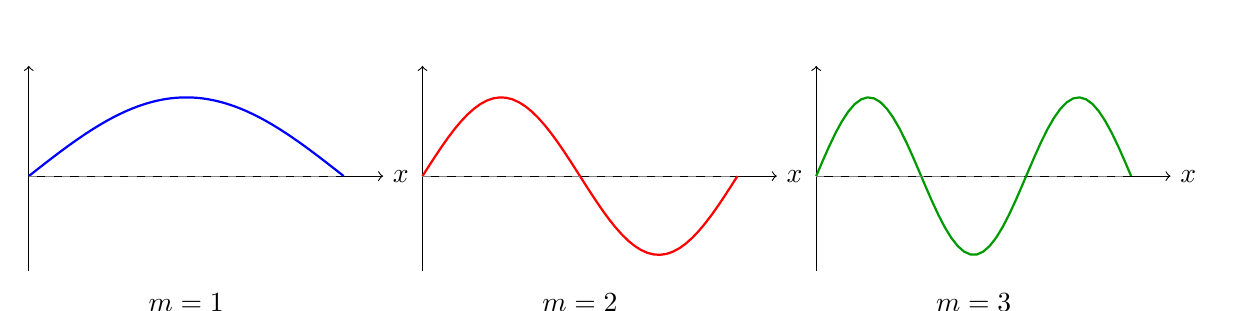
\begin{tikzpicture}[scale=1]
% m=1
\begin{scope}[xshift=0cm]
\draw[->] (0,0) -- (4.5,0) node[right] {$x$};
\draw[->] (0,-1.2) -- (0,1.4);
\draw[thick,blue] plot[domain=0:4,samples=50] (\x,{sin(45*\x)});
\draw[dashed,gray] (0,0) -- (4,0);
\node at (2,-1.6) {$m=1$};
\end{scope}
% m=2
\begin{scope}[xshift=5cm]
\draw[->] (0,0) -- (4.5,0) node[right] {$x$};
\draw[->] (0,-1.2) -- (0,1.4);
\draw[thick,red] plot[domain=0:4,samples=50] (\x,{sin(90*\x)});
\draw[dashed,gray] (0,0) -- (4,0);
\node at (2,-1.6) {$m=2$};
\end{scope}
% m=3
\begin{scope}[xshift=10cm]
\draw[->] (0,0) -- (4.5,0) node[right] {$x$};
\draw[->] (0,-1.2) -- (0,1.4);
\draw[thick,green!60!black] plot[domain=0:4,samples=50] (\x,{sin(135*\x)});
\draw[dashed,gray] (0,0) -- (4,0);
\node at (2,-1.6) {$m=3$};
\end{scope}
\end{tikzpicture}
\caption{Eigenfunctions $\sin(m\pi x/L)$ for $m=1,2,3$. The 2D eigenfunctions are products: $\sin(m\pi x/L_x)\sin(n\pi y/L_y)$. Higher modes oscillate more rapidly and contribute less to the solution because their eigenvalues $\lambda_{mn} \propto m^2 + n^2$ appear in the denominator.}
\label{fig:modes}
\end{figure}

The eigenfunctions form an orthonormal basis for the solution space. Each eigenfunction satisfies the Laplacian eigenvalue problem with eigenvalue $-\lambda_{mn}$ where:
\begin{equation}
\lambda_{mn} = \frac{m^2\pi^2}{L_x^2} + \frac{n^2\pi^2}{L_y^2}
\end{equation}
Substituting the expansion into the Poisson equation and projecting onto each eigenfunction yields the modal amplitudes:
\begin{equation}
A_{mn} = -\frac{F_{mn}}{\lambda_{mn}}, \quad \text{where } F_{mn} = \frac{4}{L_x L_y} \int_0^{L_x}\int_0^{L_y} f(x,y) \sin\left(\frac{m\pi x}{L_x}\right) \sin\left(\frac{n\pi y}{L_y}\right) dy\, dx
\end{equation}
The coefficient $F_{mn}$ is the projection of the source term $f$ onto each eigenfunction. This is precisely what FFT-based solvers compute numerically: the Discrete Fourier Transform projects the discretized $f$ onto sinusoidal basis functions, and division by the eigenvalues $\lambda_{mn}$ yields the solution coefficients.


%%%%%%%%%%%%%%%%%%%%%%%%%%%%%%%%%%%%%%%%%%%%%%%%%%%%%%
% End of Chapter 2: Mathematical Foundation

\end{document}